% PREAMBLE
%%%%%%%%%%%%%%%%%%%%%%%%%%%%%%%%%%%%%%%%%%%%%%%%%%%%%%%%%%%%%%%%%%%%%%%%%%%%%%%%%%%%%%%%%%%%%%%%%%%%%%%%
%%%%%%%%%%%%%%%%%%%%%%%%%%%%%%%%%%%%%%%%%%%%%%%%%%%%%%%%%%%%%%%%%%%%%%%%%%%%%%%%%%%%%%%%%%%%%%%%%%%%%%%%
\documentclass[10pt]{article}
\usepackage{geometry}                	% See geometry.pdf to learn the layout options. There are lots.
\geometry{top=1.0in, bottom=1.0in, left=1.0in, right=1.0in}                   	% ... or a4paper or a5paper or ...
%\geometry{landscape}                	% Activate for for rotated page geometry
\usepackage{fancyhdr} 			% This should be set AFTER setting up the page geometry
\pagestyle{fancy} 				% options: empty , plain , fancy
\renewcommand{\headrulewidth}{0pt} % customise the layout...
\lhead{}\chead{}\rhead{}
\lfoot{}\cfoot{\thepage}\rfoot{}
%\usepackage[parfill]{parskip}   	   	% Activate to begin paragraphs with an empty line rather than an indent
\usepackage{graphicx}
\usepackage{amssymb}
\usepackage{epstopdf}
\usepackage{booktabs} 			% for much better looking tables
\usepackage{array} 				% for better arrays (eg matrices) in maths
\usepackage{paralist} 			% very flexible & customisable lists (eg. enumerate/itemize, etc.)
\usepackage{verbatim}			% adds environment for commenting out blocks of text & for better verbatim
\usepackage{subfigure} 			% make it possible to include more than one captioned figure/table in a single float
\usepackage{algorithmic}
\DeclareGraphicsRule{.tif}{png}{.png}{`convert #1 `dirname #1`/`basename #1 .tif`.png}
\usepackage{sectsty}
%\allsectionsfont{\sffamily\mdseries\upshape} 	% (See the fntguide.pdf for font help)
%\usepackage[utf8]{inputenc} 		% Any characters can be typed directly from the keyboard, eg éçñ
%\usepackage{textcomp} 		% provide lots of new symbols
\usepackage{graphicx}  			% Add graphics capabilities
\usepackage{epstopdf} 			% to include .eps graphics files with pdfLaTeX
\usepackage{flafter}  			% Don't place floats before their definition
\usepackage{amsmath,amssymb} 	% Better maths support & more symbols
\usepackage{bm}  				% Define \bm{} to use bold math fonts
\usepackage{memhfixc}  			% remove conflict between the memoir class & hyperref
%\usepackage{pdfsync}  			% enable tex source and pdf output syncronicity
\usepackage[pdftex,bookmarks,colorlinks,breaklinks]{hyperref}  % PDF hyperlinks, with coloured links
\hypersetup{linkcolor=black,citecolor=black,filecolor=black,urlcolor=black} % black links, for printed output
\usepackage{cite}
\usepackage{mathtools}
\usepackage{subfigure}			% for putting figures "side-by-side"
%\usepackage{sidecap}			% sidecaption figures
\usepackage{wrapfig}
\usepackage{caption}
\usepackage{multicol}

%\makeatletter
%\newenvironment{tablehere}
  %{\def\@captype{table}}
  %{}

%\newenvironment{figurehere}
 % {\def\@captype{figure}}
 % {}
%\makeatother


% Title Page
\title{\textbf{CBEMD} Parallelized Molecular Dynamics in Various Thermodynamic Ensembles}
\author{Nathan A. Mahynski, George A. Khoury, Carmeline J. Dsilva, \\
Arun Prabhu, Francesco Ricci, and Junyoung Park}
\date{}

\begin{document}
\maketitle
\begin{figure}[htbp]
   \centering
   
\includegraphics[width=2.5in]{princeton.jpg}
\end{figure}
\thispagestyle{empty}
\newpage
\setcounter{page}{1}
\pagenumbering{arabic}
\newpage

\section{Project Overview}
We propose to develop a software package to perform parallelized molecular dynamics (MD) calculations for several different thermodynamic ensembles. Molecular dynamics is a technique commonly used to simulate the motions of a system of interest on a microscopic level; one can then calculate macroscopic properties from the microscopic features of this system. Properties such as diffusion coefficients, specific heats, and chemical potentials, which are often difficult or impossible to measure in experiment, are commonly calculated in MD.  Because of the myriad of properties that can be calculated, MD has applications such fields as material science, pharmaceutical design, cellular biology, thermodynamics, and fluid mechanics.  Due to its relative simplicity and its ability to be massively parallelized, MD is a common but powerful tool for many scientists and engineers today.

\subsection{Background on Molecular Dynamics}
MD first initializes a system of particles, usually thought of as atoms, molecules, or another relevant (molecular-scale) group.  Given an interaction potential $V (\overrightarrow{r})$ between these particles, MD integrates Newton's equation of motion, $\overrightarrow{F}=m\overrightarrow{a}$, forward in time.  Thus, the flow of the program follows a well defined set of steps:
\begin{enumerate}
    \item Initialize positions and choose a timestep, $dt$
    \item Calculate the forces $\overrightarrow{F} =  -\nabla V (\overrightarrow{r}) $
    \item Numerically integrate to calculate the displacement over $dt$, using the relationships $\overrightarrow{F}=m\overrightarrow{a}$, $\overrightarrow{a} = \frac{\overrightarrow{v}}{dt}$, and $\overrightarrow{v} = \frac{\overrightarrow{r}}{dt}$
    \item Update positions and time
    \item Repeat from step 2 until final time
\end{enumerate}

Users of any molecular dynamics program must provide the initial configuration for the particles.  In our project, we will provide an additional user interface to generate some configurations based on an interactive questionnaire. The user must also supply the relevant potential function $V$. Different potential functions can be used to describe the system at different levels of accuracy. These functions typically try to capture van der Waals interactions due to coupling of electron clouds, but can also incorporate additional effects, such as long range charge-charge interactions and solvation interactions (Debye screening effects). Our project will provide an easily extensible interface so that the user can incorporate additional interactions.

For numerical stability, the timestep $dt$ is typically on the order of a femtosecond. The longest simulations reported for macromolecules such as proteins are on the microsecond timescale, but such lengthy simulations can require specialized supercomputing hardware such as ANTON or GPUs. Although the time integration must be done sequentially, at each step, the evaluation of the potential energy and forces can be parallelized, which is the primary reason MD has been so successful on large computer clusters.

%A typical MD cascade involves the minimization of the initial configuration of a system to a local minimum. Next, the system is heated, which may involve restraining the atoms of the system, or gently over longer periods of time. The system is next equilibrated and submitted for production, where temperatures, pressures, energies, and other properties intrinsic to the simulation are recorded. Higher order properties of the system are usually recorded here as well. Temperature controls the velocity of the system, and can be related to velocity using the equipartition theorem and the Maxwell-Boltzmann distribution.

There are many different numerical integration algorithms that have been developed, each with a slightly different purpose and numerical stability.  These include (but are not limited to):

\begin{enumerate}
    \item Verlet
    \item Velocity Verlet
    \item Leapfrog
\end{enumerate}

The above algorithms are designed to maintain constant energy ($E$), volume ($V$), and number of particles ($N$).  This NVE ensemble is known in thermodynamics as the {\em microcanonical ensemble}.
% and reaches equilibrium when the entropy of the system reaches a maximum.
Although this ensemble is the simplest to analyze in a thermodynamic framework, it is almost never applicable to real world problems.
Other widely used ensembles include the {\em canonical ensemble} (NVT) and the {\em isothermal-isobaric ensemble} (NPT), which is the often the most representative of experimental conditions.
%These ensembles correspond to a maximization of entropy subject to constraints and their equilibrium corresponds to Helmholtz and Gibbs free energy, respectively.
Our project will incorporate these additional ensembles, which corresponds to implementing different integrators.

Several existing MD packages, such as HOOMD, LAMPS, GROMACS, and NAMD, incorporate such ensembles. Members of our group use some of these codes in our every day research, but we do not know much about their internal structure. Therefore, it is a prudent exercise to develop our own codebase with a well-written interface that we can each extend for our custom applications.

\subsection{Molecular Dynamics Codebase}
In our project, we plan to develop the molecular dynamics codebase \textbf{CBEMD}. This codebase will be written in C++ and Python. The bulk of the code will be written in C++, a language that maintains good performance while affording us the conveniences of object oriented programming and relative ease of parallelization with MPI. The code will be linked to boost to utilize a number of special string manipulation features for data parsing, but will otherwise be developed from scratch. Testing will be done using Googletests and potentially python unittests if we are able to wrap the C++ with Python by using SWIG.

We will have two levels of user interfaces.  The first and more basic interface will be through a C++ driver program with command line input.  A more user friendly interface will be written in Python, where a user can interactively set up their simulation. Documentation of the codebase will be done using Doxygen.

%We plan to develop this codebase, and likely extend this in our own research. If successful, we potentially plan to publish it as an open-source alternative to those many that already exist.

%For example, one may be able to measure the unfolding rate of a protein that unfolds slightly above room temperature experimentally. A thermophilic protein, one that can resist degradation due to increased temperatures as a result of evolutionary fitness, may unfold at temperatures higher than room temperature. Experiments are time consuming and costly, and therefore one would
%Alternatively, when designing a possible drug to bind to and inhibit a target receptor, it would be prohibitively expensive and time consuming ..

\section{Flowchart}
A flowchart of our molecular dynamics program is presented in Figure \ref{fig:flowchart}.
\begin{figure}[h]
\centering
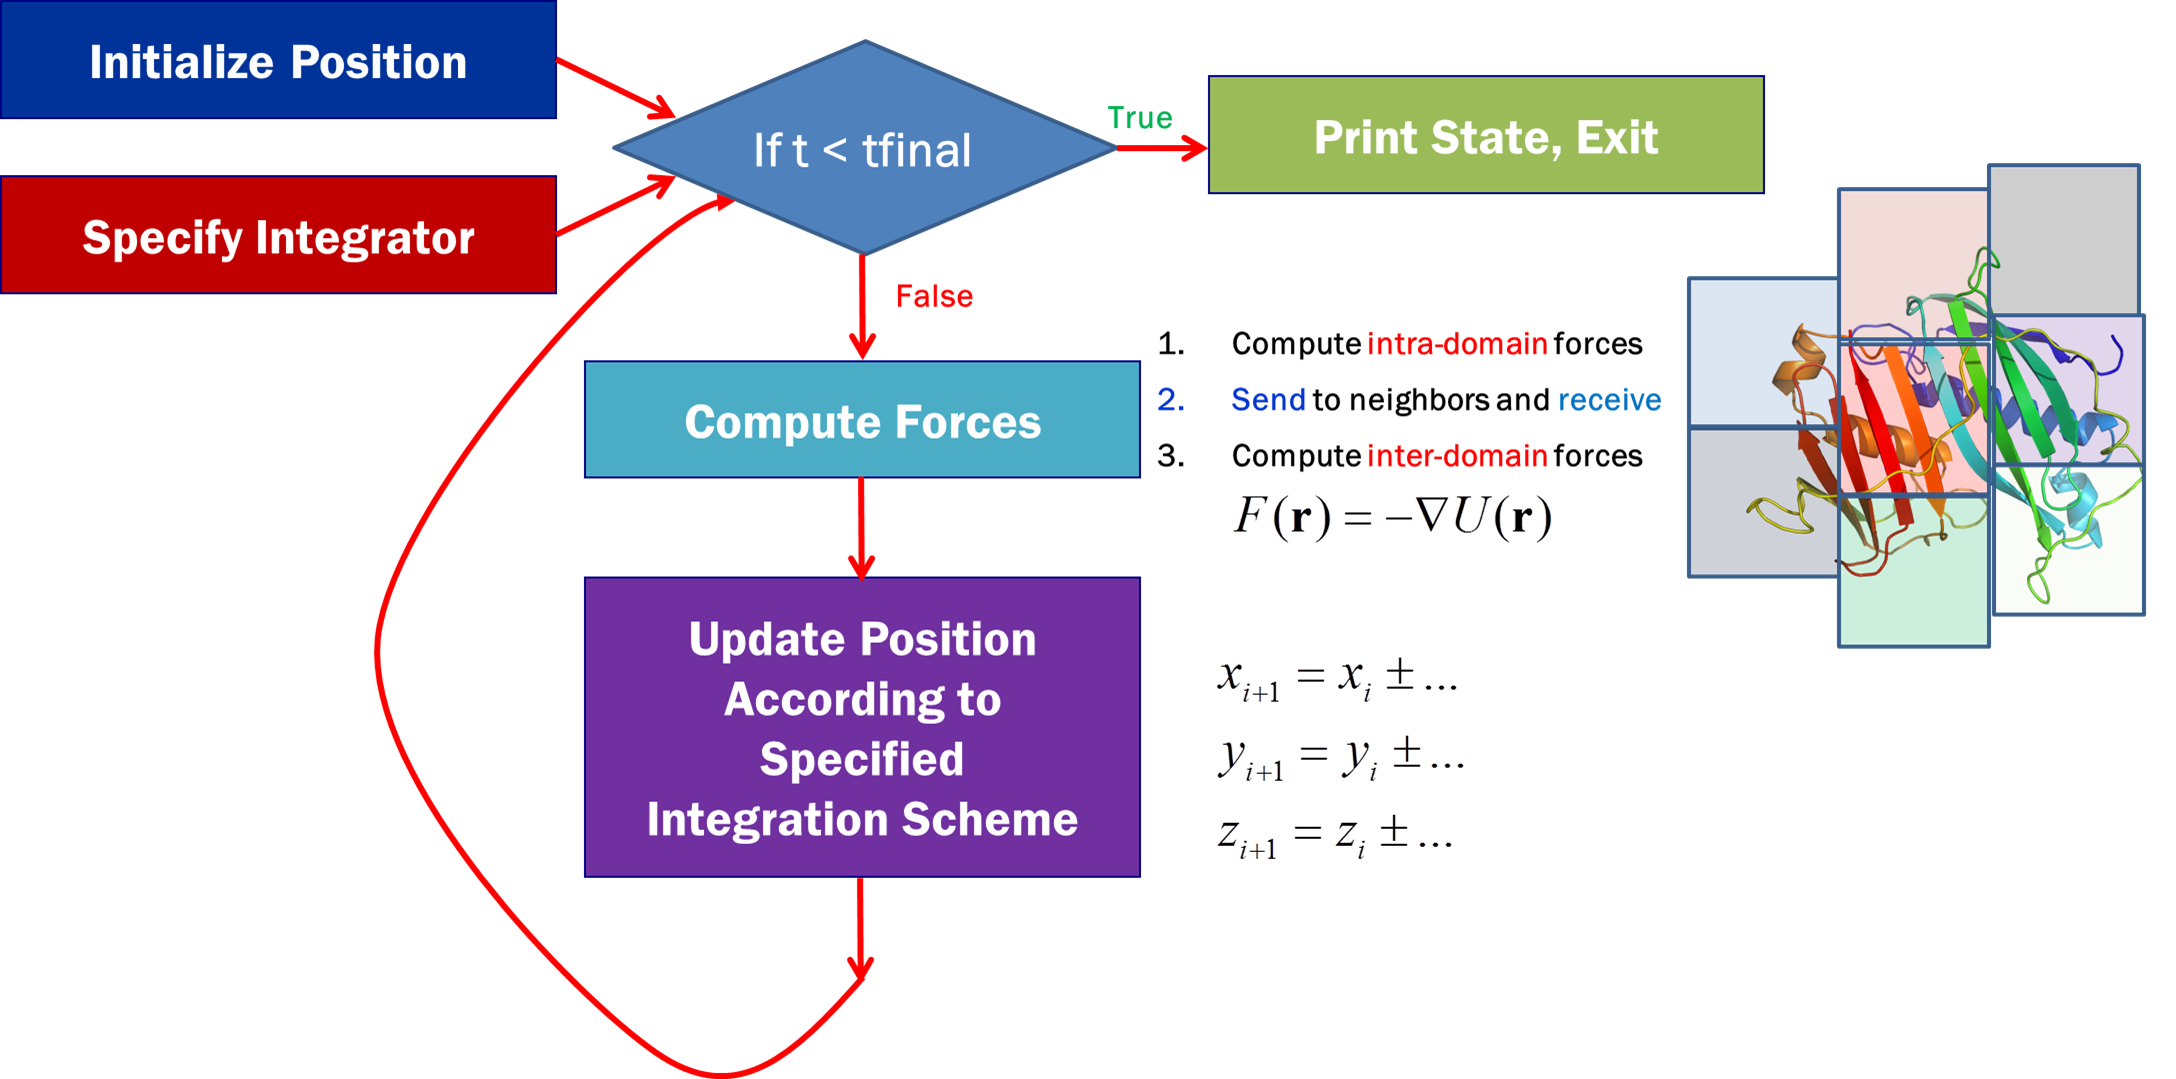
\includegraphics[width=0.75\textwidth]{flowchart.png}
\caption{Visual representation of the flow of the molecular dynamics program. First, the initial system configuration and other parameters of the simulation are provided, one of which is $t_{final}$, the time for which to run the simulation. For each integration step, the forces on each particle are calculated and used to update the positions of the particles.}
\label{fig:flowchart}
\end{figure}

% flow of MD program
% need to talk to nate about making an image. when he describes it for a few minutes, I'll make a cool figure.
% handling bonds, neighbor lists to accelerate
\section{User Interface}
The advanced user interface will be implemented using Python. It will pose a questionnaire in order to populate an xml input file.  More advanced users can simply provide this xml file and call the program from the command line.  The latter option will be contained in our alpha release.  Using SWIG (www.swig.org), we will expand our codebase so that a user can provide a Pythonic input file instead of a C++ driver program; this will be incorporated in our beta or final release version.

% swig/pythonic
% alternatively can make a very simple c++ code using built in functions

\section{Schedule \& Assignments}
\subsection{Design Document}
Mr. Khoury and Mr. Mahynski will produce the design document and present it to the group. The group will make edits, and it will be submitted. (11/23/12)

\subsection{First Presentation}
Mr. Khoury will produce the design presentation and present it to the group. The group will make edits, and it will be presented. (11/26/12)

\subsection{Interface}
Before any programming is done, we will design an efficient interface to facilitate group work. The general components will consist of classes for the major components involved in MD including:
\begin{enumerate}
	\item{System} \par This class will contain all pertinent information about the simulation box such as temperature, pressure, and box dimensions.  This class will also store information about atoms and bonds.  When using MPI, the simulation box will be decomposed into ``subsystems," each of which exists on a unique processor. %and is responsible for simulating a given region of the box.  %These will be designed such that only nearest neighbors will need to communicate information.
	\item{Atom} \par This will be a structure, i.e. no functions will be stored in this class, because this is the main ``workhorse" of the program and will need to be passed repeatedly between processors to communicate requisite information for the integration step.  Therefore, this class will only store critical information and base data types easily passed through MPI.  This includes information such as positions, velocities, and particle types that are necessary for the force calculations.
	\item{Bond} \par Bonds are by far the largest complication in MD, because global indices must be tracked to manage what atoms are bonded to each other (since atoms participating in a bond may exist on different processors).  The Bond class will be an abstract base class which allows users to define different types easily, requiring only that each defined type have an energy and force calculation.  Parameters involved in a bond ``type" will be set by the user and available on all processors at all times so such information need not be passed; the only information necessary to compute bonding contributions an array of bonded pairs of atoms and their ``type."  The bond type is an internally indexed quantity that is hidden from the user, and is accessed by a name (string).
	\item{Integrator} \par There are many different integrators that exist which correspond to different ensembles.  This will be an abstract base class, allowing the user to expand on what we develop and add new integrators in the future.  We plan to implement integrators for the microcanonical  (NVE), canonical (NVT), and isothermal-isobaric ensemble (NPT).  For the NVE ensemble, integrators include Verlet, Velocity Verlet, and the Leapfrog algorithm.  Thermostats and barostats (required for the NVT and NPT ensembles) include Nose-Hoover and Anderson.
	\item{Pair Potentials} \par This class defines the interaction potential $V$ between particles. As it is the most common, we will provide a shifted Lennard-Jones pair potential, $V(r) = 4\epsilon \left( \left( \frac{\sigma}{r-\Delta} \right)^{12} - \left( \frac{\sigma}{r - \Delta} \right)^{6} \right)$. Users can easily add additional pair potentials.
\end{enumerate}

\subsection{Alpha Version}
In this release, the MD program will be able to read in an initial configuration of atoms, and utilize at least one of the integrators aforementioned to perform serial MD calculations.

Mr. Mahynski will develop the interface (classes, see above) and overall structure of the codebase, as well an the initialization routine to read from a standardized input (an xml file).  He will also be responsible for developing the derived Atom class for MPI to properly pass this information. (12/1/12)

Mr. Khoury will develop user interface using SWIG (Pythonic) or Python and provide a some basic proof of concept; prior to this, our interface will be through a C++ driver program. Mr. Khoury will experiment with SWIG to determine whether we should use SWIG for the user interface, or use Python directly instead. (12/1/12)

Mr. Park and Mr. Ricci will be responsible for the force calculation which is required in all integrators.  This will require a fair amount of work to implement this in parallel (using MPI) given an arbitrary domain decomposition. (12/5/12)

Mr. Prabhu will be responsible for creating an algorithm to do an ``optimal" domain decomposition given an arbitrary number of processors, and assist in implementing the force calculation.  (12/1/12)

Mrs. Dsilva will be responsible for handling pair potential classes, bonds, and integrators.  (12/1/12)

\subsection{Beta Version}
In this release, the integrators will be finished and tested.  MPI calls and force calculations will be finished and tested.

Mr. Khoury will refine the Pythonic interface either directly in Python, or using Swig. Note, that Mr. Khoury will be away in Rome, Italy and Gaeta, Italy from 12/7/12/ until 12/14/12 for the CASP10 conference and will have limited access to computing resources during that time.   (12/15/12)

Mrs. Dsilva will expand on the project goals and develop a routine to measure and externally optimize forces obtained during the run for the purpose of locating saddle points in the energy surface.  She will also handle output of system configurations for visualization.  (12/31/12)

Mr. Prabhu, Mr. Mahynski, Mr. Khoury and Mr. Ricci will  be responsible for optimizing the code, and profiling. (12/15/12)

Mr. Park will be responsible for using Google tests to test the C++ components. Mr. Khoury will help Mr. Park with this. (12/31/12)

Mr. Khoury will be responsible for python unittests to test the user interface. (12/31/12)

\subsection{Final Version}
Our final version will include integrators for all ensembles, a refined method of visualization, and final tests involving MPI.  We will validate our codebase against known results for Lennard-Jones fluids and binary spheres.  Our codebase will incorporate a convenient, Pythonic user interface.

\subsection{Code Features}
The above was a description of the different deliverables from the codebase standpoint that we propose to undertake. Here, we describe several features that we hope the final code will have.
\begin{enumerate}
    \item The program should be able to easily be extended to use arbitrary interparticle potentials as long as they conform to the abstract base class. As an example, we will use Lennard-Jones.
    \item The MD program should be able to print out binary files that can be visualized using VMD or other visualization programs that exist, as well as xml snapshots.
    \item The MD program should be able to stably run for an arbitrary length of time on an arbitrary number of processors.
    \item Force constants will be able to be performed in parallel.
    \item The MD program should able to be started using two mechanisms. First, through reading an xml-based input file, or by using a python script with an easily usable user interface.
    \item The final version should be able to handle bonds of an arbitrary nature as long as they conform to the bond abstract base class. Because of this feature, our MD code can be extended to arbitrarily complex molecules.
\end{enumerate}
\end{document}

